\documentclass[11pt, oneside]{article}   	% use "amsart" instead of "article" for AMSLaTeX format
\usepackage{geometry}                		% See geometry.pdf to learn the layout options. There are lots.
\geometry{letterpaper}                   		% ... or a4paper or a5paper or ... 
%\geometry{landscape}                		% Activate for for rotated page geometry
%\usepackage[parfill]{parskip}    		% Activate to begin paragraphs with an empty line rather than an indent
\usepackage{graphicx}				% Use pdf, png, jpg, or eps� with pdflatex; use eps in DVI mode
								% TeX will automatically convert eps --> pdf in pdflatex		
\usepackage{amssymb}
\usepackage{amsmath}
\usepackage{parskip}

\graphicspath{{/Users/telliott_admin/Dropbox/Tex/png/}}

\title{Puzzles}
\date{}
\begin{document}
\maketitle
\large

\begin{center} 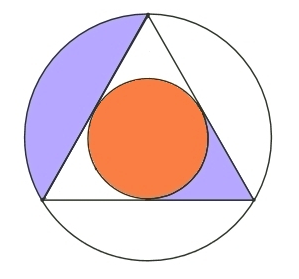
\includegraphics [scale=0.4] {areapuzzle1.png} \end{center}

I found some puzzles online.  The first challenge is to show that the area of the orange inner circle is equal to the total of the two areas shaded blue. The triangle is equilateral.

% http://johncarlosbaez.wordpress.com/2014/01/12/geometry-puzzles/

We can find a relationship between the length of the side of the triangle and the radius for each circle, but it turns out we don't actually need to.

\begin{center} 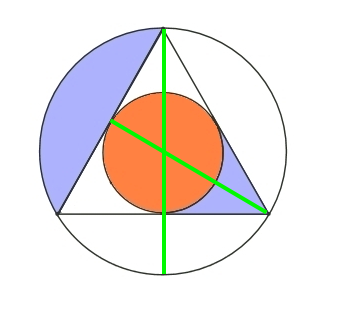
\includegraphics [scale=0.4] {areapuzzle1b.png} \end{center}

Let the radius of the large circle be $R$.  Draw the vertical diameter of the larger circle so as to divide the triangle into two identical halves.  The angle between the diameter and the adjacent side of the triangle is $t = \pi/6$.

Draw the radius of the small circle $r$ so that it bisects the side of the triangle.  This forms a right triangle containing angle $t$ where $r = R \sin t$ or 

\[ 2r = R \]

\begin{center} 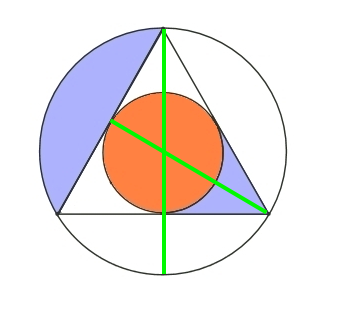
\includegraphics [scale=0.4] {areapuzzle1b.png} \end{center}

The area of three times the larger purple sector is

\[ 3 A_L = A_C - A_T \]

We can scale the figure however we like (in particular it would be convenient to set $s=1$), but let's leave it in this form for now.  On to the inner circle.


If the area of the small circle is $A_c$, then the area of three copies of the smaller purple sector is

\[ 3A_S = A_T - A_c \]

What we are asked to show is that
\[ A_L + A_S = A_c \]
\[ 3A_L + 3A_S = 3A_c \]
\[ A_C - A_T + A_T - A_c = 3A_c \]
\[ A_C = 4 A_c \]
 
\[ R^2 = 4r^2 \]
\[ 2r = R \]

This is what we showed at the top, so we're done.

\subsection*{}

\begin{center} 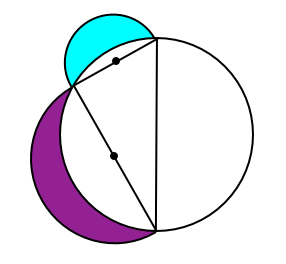
\includegraphics [scale=0.75] {areapuzzle2.png} \end{center}

A right triangle is inset in a (larger) circle, and the two "lunes" are drawn, which are the colored crescent areas peaking out behind the circumference of the large circle.  These are drawn with centers on the sides of the triangle, as indicated by the points.  We are asked to show that the sum of the colored areas is equal to the area of the triangle.

It is not given that the third side of the right triangle is a diameter of the circle, but I say that it is true.  Assume that it is not the case.  Then consider the right angle and choose one of the other vertices and draw the triangle with the true diameter, having as its third vertex a different point than the one shown.  This second triangle will be a right triangle.  But there cannot be two right triangles containing the two points and both with their third vertex on the circle.  Hence, the line shown is a diameter of the circle.

So now, call the radius of the blue circle $b$ and the radius of the purple circle $p$, and the radius of the large circle $r$.  By similar triangles, the distance between the two marked points is equal to $r$ and so

\[ b^2 + p^2 = r^2 \]
\[ \frac{\pi}{2} b^2 + \frac{\pi}{2} p^2 = \frac{\pi}{2} r^2 \]

The area of the larger semicircle is equal to the sum of the areas of the smaller semicircles.

From the area of the large semicircle, subtract the areas that are shared with the two smaller semicircles, leaving the triangle.  Similarly, subtract from each small semicircle the area that is shared, leaving the colored areas behind.  The areas that are not shared have the same relationship as the whole semicircles.





\enddocument{}